%rules.tex
\documentclass[a4paper, 10pt]{scrartcl}

%importing german packages%
\usepackage[ngerman]{babel}
\usepackage[utf8]{inputenx}
\usepackage[T1]{fontenc}

\usepackage{amsmath}
\usepackage{xcolor}
\usepackage{hyperref}
\usepackage{listings}
\usepackage{enumerate}
\usepackage{graphicx}
\usepackage{fancyhdr}
\usepackage{sidecap}
\usepackage{placeins}
\usepackage{wrapfig}
\usepackage[export]{adjustbox}
\usepackage{tikz-uml}

\sidecaptionvpos{figure}{t}

\pagestyle{fancy}
\fancyhf{}
\lhead{Julian Sehbaoui}
\chead{\glqq Schach.py\grqq{}}
\rhead{Luisengymnasium Bergedorf}
\rfoot{Seite \thepage}
\renewcommand{\headrulewidth}{2pt}

%setting document attributes for the titlepage%
\title{Informatik Dokumentation\\Die Regeln des Schach}
\author{Julian Sehbaoui}
\date{\today}

%begin the document
\begin{document}
\begin{titlepage}
    \maketitle
    \centering
    \url{https://github.com/JSehbaoui/Chess_Python}\\
     \vspace{5pt} 
    
\includegraphics[scale=0.35]{assets/luisengymnasium.png}\\
     \vspace{5pt} 
    
    Made with \LaTeX{}
\end{titlepage}

\tableofcontents

\pagebreak

\section{Das Spielprinzip}
Ein Schachspiel wird zwischen zwei Gegnern ausgetragen, die ihre Spielfiguren auf einem quadratischen Spielbrett ziehen. 
Das Ziel des Spiels für beide Spieler ist es den gegnerischen König „Schachmatt“ zu setzten. Dieser Zustand ist erreicht, wenn der gegnerische Spieler keine Möglichkeit hat, den König mit dem nächsten Zug aus dem „Schach“ (angegriffener Zustand des Königs) zu bewegen. 
Falls es für keinen der Beiden Spieler möglich ist den Gegner Schachmatt zu setzten, wird das Spiel mit einem Remis (=Unentschieden/Gleichstand) beendet.

\section{Anfangsstellung der Figuren}
Das Schachbrett besteht aus einem 8x8 Gitter mit 64 gleichgroßen Quadraten, welche abwechselnd hell und dunkel sind (meist weiß und schwarz).
Die Spieler positionieren sich gegenüber voneinander, sodass bei beiden Spielern ein weißes Feld in der unteren rechten Ecke vorhanden ist.
Zu Beginn des Spiels hat jeder Spieler 16 Figuren; Ein Spieler die die Hellen (weiß) und einer die Dunklen (schwarz).
Beide Spieler starten mit 8 Bauern, 2 Türmen, 2 Springern, 2 Läufern, einer Dame und einem König.
Die Figuren sind wie folgt anzuordnen:

\begin{figure}[h]
        \centering
        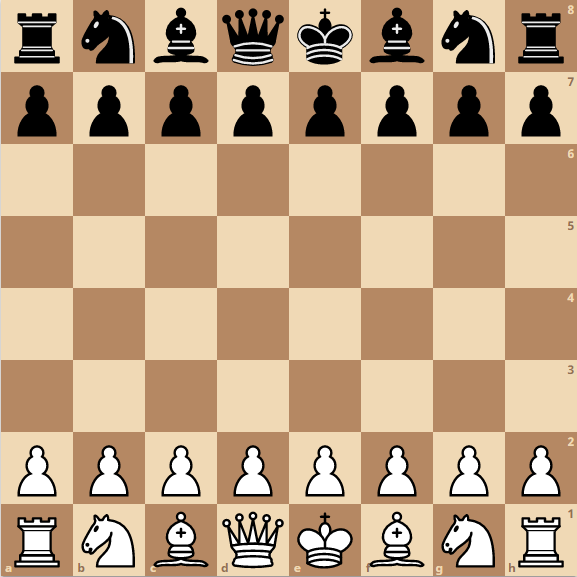
\includegraphics[scale=0.5]{assets/chess-opening.png}
        \caption{Anfangsaufstellung der Schachfiguren im Standardschach}
\end{figure}


Die senkrechten Spalten sind die „Linien“, die waagerechten Zeilen sind die „Reihen“ und die gradlinige Folge der Felder, die sich an den Ecken Berühren sind die „Diagonalen“.

\section{Gangart der Figuren}
Allgemeingültige Regeln sind folgende:
\begin{itemize}
        \item Eine Figur darf nicht auf das Feld einer verbündeten Figur ziehen
        \item Es ist nicht möglich eine Figur durch ein Feld hindurch zu ziehen, welches von einer anderen Figur besetzt ist (Ausnahme siehe 3.3.4.)
        \item Wenn eine Figur auf ein Feld zieht, welches von einer gegnerischen Figur besetzt ist, dann wird die Gegnerfigur geschlagen (=entfernt)
        \item Keine Figur darf einen Zug machen, welcher den eigenen König einem Schachgebot aussetzt oder ihn in einem Schachgebot stehen lässt.
    
\end{itemize}

\subsection*{Läufer}
\begin{SCfigure}[4][h]
        \caption{\protect\rule{0ex}{4ex}
        Der Läufer darf auf ein beliebiges 
        Feld entlang der Diagonale ziehen, auf der er steht.
        }
        
\includegraphics[width=0.15\textwidth]{assets/bishop_split.png}
\end{SCfigure}

\pagebreak

\FloatBarrier
\subsection*{Turm}
\begin{SCfigure}[4][h]
        \caption{\protect\rule{0ex}{4ex}
        Der Turm darf auf ein beliebiges Feld 
        entlang der Linie oder der Reihe ziehen, auf der er steht.
        }
        
\includegraphics[width=0.15\textwidth]{assets/rook_split.png}
\end{SCfigure}

\FloatBarrier

\subsection*{Dame}
\begin{SCfigure}[4][h]
        \caption{\protect\rule{0ex}{4ex}
        Die Dame darf auf ein beliebiges Feld 
        entlang der Linie, Reihe oder Diagonalen ziehen, auf der die steht.
        }
        
\includegraphics[width=0.15\textwidth]{assets/queen_split.png}
\end{SCfigure}

\subsection*{Springer}
\begin{SCfigure}[4][h]
        \caption{\protect\rule{0ex}{4ex}
        Der Springer darf auf eines der Felder ziehen, 
        die seinem Standfeld am nächsten, aber nicht auf gleicher Linie, 
        Reihe oder Diagonalen mit diesem liegen.
        }
        
\includegraphics[width=0.15\textwidth]{assets/knight_split.png}
\end{SCfigure}

\subsection*{Bauer}

\begin{wrapfigure}{l}{0.28\textwidth}
        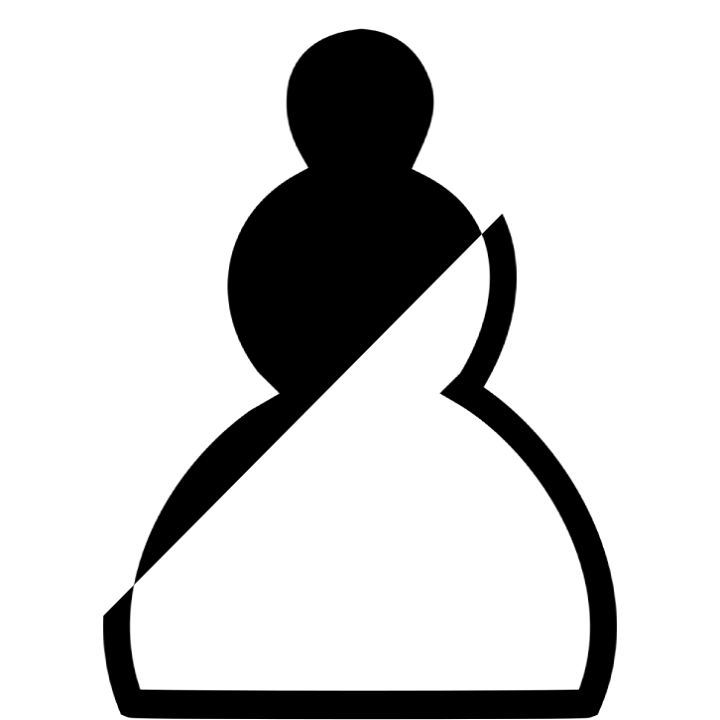
\includegraphics[width=0.15\textwidth, right]{assets/pawn_split.png}
\end{wrapfigure}
Der Bauer darf
\begin{itemize}
        \item vorwärts auf das unbesetzte Feld direkt vor ihm auf derselben Linie ziehen
        \item in seinem ersten Zug entweder wie unter (a) beschrieben ziehen oder um zwei Felder entlang derselben Linie vorrücken, vorausgesetzt, dass beide Felder frei sind, oder
        \item auf ein von einer gegnerischen Figur besetztes Feld diagonal vor ihm auf einer benachbarten Linie ziehen, indem er jene Figur schlägt.
        \item sobald er diejenige Reihe erreicht hat, die am weitesten von seinem Ursprungsfeld entfernt ist, muss er sich als Teil desselben Zuges gegen eine Dame, einen Turm, einen Läufer oder einen Springer derselben Farbe austauschen. Die Auswahl des Spielers ist nicht auf bereits geschlagene Figuren beschränkt. Dieser Austausch eines Bauern für eine andere Figur wird «Umwandlung» genannt, und die Wirkung der neuen Figur tritt sofort ein.
\end{itemize}


\subsection*{König}

\begin{wrapfigure}{l}{0.28\textwidth}
        
\includegraphics[width=0.15\textwidth, right]{assets/king_split.png}
\end{wrapfigure}
Es gibt zwei verschiedene Arten den König zu ziehen:
\begin{enumerate}
        \item Er zieht auf ein beliebiges angrenzendes Feld, das nicht von einer oder mehreren gegnerischen Figuren angegriffen wird. Von den gegnerischen Figuren gilt, dass sie ein Feld auch dann angreifen, wenn sie selbst nicht ziehen können. Oder
        \item er «rochiert». Die «Rochade» ist ein Zug des Königs und eines gleichfarbigen Turmes auf der gleichen Reihe. Sie gilt als ein einziger Zug und wird folgendermaßen ausgeführt: Der König wird von seinem Ursprungsfeld um zwei Felder in Richtung des Turmes hin versetzt, dann wird dieser Turm auf das Feld gesetzt, das der König soeben überquert hat.
        \begin{enumerate}
                \item Die Rochade ist regelwidrig:
                \begin{enumerate}
                        \item wenn der König bereits gezogen hat, oder
                        \item mit einem Turm, der bereits gezogen hat.
                \end{enumerate}
                \item Die Rochade ist vorübergehend verhindert,
                \begin{enumerate}
                        \item wenn das Standfeld des Königs oder das Feld, das er überqueren muss, oder sein Zielfeld von einer oder mehreren gegnerischen Figuren angegriffen wird,
                        \item wenn sich zwischen dem König und dem Turm, mit dem rochiert werden soll, irgendeine Figur befindet.
                \end{enumerate}
        \end{enumerate}
\end{enumerate}
Ein König «steht im Schach», wenn er von einer oder mehreren gegnerischen Figuren angegriffen wird, auch wenn diese selbst nicht ziehen können.

\section{Ende der Partie}
Eine Partie endet entweder durch ein „Schachmatt“ oder durch ein „Remis“ (siehe 3.1.).
Eine Partie kann auch durch eine Übereinstimmung beider Spieler mit einem Remis entschieden werden. 
Ein Ende Partie ist auch durch eine dreifach wiederholte identische Zugfolge mit einem Remis zu beenden. 
Falls 50 Züge ohne einen Bauernzug oder das schlagen einer Figur vergehen, ist dies ebenfalls ein Unentschieden.
\end{document}